\documentclass{article}

%=====================================================================
%============================= packages ==============================

%\usepackage{geometry}
\usepackage{amsmath}
\usepackage{amssymb}
\usepackage{stmaryrd}
\usepackage{fancyhdr}
\usepackage{natbib}
\usepackage[normalem]{ulem}
\usepackage{examples-slim}
\usepackage{xcolor}
\usepackage{graphicx}
\usepackage{float}
\usepackage{multirow}
\usepackage{booktabs}
\usepackage{colortbl}
\usepackage{caption}
\usepackage{subcaption}
\definecolor{black}{rgb}{0,0,0}
\usepackage[colorlinks, linkcolor=black, urlcolor=black, citecolor=black]{hyperref}

\bibpunct[; ]{(}{)}{;}{a}{}{,}  % natbib citation style

%=====================================================================
%========================= cross-references ==========================

% Flexible sec/fig/tbl/def cross-refs.
\newcommand{\Secref}[1]{Section~\ref{#1}}
\newcommand{\secref}[1]{section~\ref{#1}}
\newcommand{\dashsecref}[2]{sections~\ref{#1}--\ref{#2}}

\newcommand{\Defref}[1]{Def.~\ref{#1}}
\newcommand{\defref}[1]{def.~\ref{#1}}
\newcommand{\Defrefc}[2]{\Defref{#1}, clause~\ref{#2}}
\newcommand{\defrefc}[2]{\defref{#1}, clause~\ref{#2}}

\newcommand{\Figref}[1]{Figure~\ref{#1}}
\newcommand{\figref}[1]{figure~\ref{#1}}
\newcommand{\dashfigref}[2]{figures~\ref{#1}--\ref{#2}}
\newcommand{\Tabref}[1]{Table~\ref{#1}}
\newcommand{\tabref}[1]{table~\ref{#1}}

% Examples:
\newcommand{\eg}[1]{(\ref{#1})}
\newcommand{\subeg}[2]{(\ref{#1}\ref{#2})}
\newcommand{\dblsubeg}[3]{(\ref{#1}\ref{#2},~\ref{#3})}
\newcommand{\dashsubeg}[3]{(\ref{#1}\ref{#2}--\ref{#3})}

% In-text citations
\newcommand{\posscitet}[1]{\citeauthor{#1}'s~(\citeyear{#1})}
\newcommand{\sposscitet}[1]{\citeauthor{#1}'~(\citeyear{#1})}
\newcommand{\possciteauthor}[1]{\citeauthor{#1}'s}
\newcommand{\spossciteauthor}[1]{\citeauthor{#1}'}
\newcommand{\pgposscitet}[2]{\citeauthor{#1}'s~(\citeyear{#1}:~#2)}
\newcommand{\secposscitet}[2]{\citeauthor{#1}'s~(\citeyear{#1}:~$\S$#2)}
\newcommand{\pgcitealt}[2]{\citealt{#1}:~#2}
\newcommand{\seccitealt}[2]{\citealt{#1}:~$\S$#2}
\newcommand{\pgcitep}[2]{(\citealt{#1}:~#2)}
\newcommand{\seccitep}[2]{(\citealt{#1}:~$\S$#2)}
\newcommand{\pgcitet}[2]{\citeauthor{#1}~(\citeyear{#1}:~#2)}
\newcommand{\seccitet}[2]{\citeauthor{#1}~(\citeyear{#1}:~$\S$#2)}

%=====================================================================
%============================ text styles ============================

\newcommand{\word}[1]{\emph{#1}}
\newcommand{\tech}[1]{\textbf{#1}}
\definecolor{maroon}{HTML}{990000}
\newcommand{\highlight}[1]{{\color{maroon}#1}}

%=====================================================================
%============================== judgments ============================

\newcommand{\bad}{\sqz{${}^\ast$}}
\newcommand{\freebad}{${}^\ast$}
\newcommand{\marked}{\sqz{${}^\#$}}
\newcommand{\freemarked}{${}^\#$}

%=====================================================================
%=============================== model ===============================


\newcommand{\tuple}[1]{\ensuremath{\left< #1 \right>}}
\newcommand{\set}[1]{\ensuremath{\left\{ #1 \right\}}}
\newcommand{\True}{\texttt{T}}
\newcommand{\False}{\texttt{F}}
\newcommand{\Reals}{\mathbb{R}}
\newcommand{\given}{\mid}
\newcommand{\Indicator}{\mathbb{I}}

\newcommand{\sem}[1]{\ensuremath{\llbracket#1\rrbracket}}
\newcommand{\States}{W}
\newcommand{\state}{w}
\newcommand{\Lex}{\mathcal{L}}
\newcommand{\LexStar}{\Lex^{\ast}}
\newcommand{\LexSet}{\mathbf{L}}
\newcommand{\Messages}{M}
\newcommand{\msg}{m}
\newcommand{\Costs}{C}
\newcommand{\Prior}{P}
\newcommand{\LexPrior}{P_{\LexSet}}

\newcommand{\listenerZero}{l_{0}}
\newcommand{\speakerOne}{s_{1}}
\newcommand{\listenerOne}{l_{1}}
\newcommand{\SpeakerK}[1][k]{S_{#1}}
\newcommand{\ListenerK}[1][k]{L_{#1}}

\newcommand{\nullmsg}{\mathbf{0}}

%=====================================================================
%============================ annotations ============================

\let\oldmarginpar\marginpar
\renewcommand{\marginpar}[1]{\oldmarginpar[\color{red}\raggedright\scriptsize #1]{\color{red}\raggedright\scriptsize #1}}

\newcommand{\textnote}[1]{{\color{red}#1}}

%=====================================================================
%============================== colors ===============================

\definecolor{lightgray}{HTML}{CCCCCC} 

\definecolor{highlightcolor}{HTML}{D95F02}
\definecolor{annotationcolor}{HTML}{777777} 
\definecolor{worldinfocolor}{HTML}{E7298A}
\definecolor{lexcolor}{HTML}{D95F02}
\definecolor{costcolor}{HTML}{A6761D}
\definecolor{defcolor}{HTML}{D95F02}
%\definecolor{hurfordcolor}{HTML}{00CC33}
\definecolor{hurfordcolor}{HTML}{1B9E77}
\newcommand{\hurford}[1]{{\relax\color{hurfordcolor}#1}}
\newcommand{\definitional}[1]{\relax{\color{defcolor}#1}}

\newcommand{\graycell}[1]{{\cellcolor[gray]{.8}#1}}

%=====================================================================
%============================== helpers ==============================

\newcommand{\porq}{p\,\word{or}\,q}
\newcommand{\pandq}{p\,\&\,q}

\newcommand{\disjlexicon}[2]{
  \left[
    \begin{array}[c]{l@{ \ \mapsto \ } l}
      \porq    & \set{#1} \\
      \pandq   & \set{#2} \\
      \nullmsg & \set{w_{1}, w_{2}, w_{3}} \\
    \end{array}
  \right]}

\newcommand{\listenerMatrix}[6]{
  \begin{array}[c]{l *{4}{r}}
    \toprule
    #1 & w_{1} & w_{2} & w_{3} \\
    \midrule
    p        & #2 \\
    q        & #3 \\              
    \pandq   & #4 \\
    \porq    & #5 \\
    \nullmsg & #6 \\
    \bottomrule
  \end{array}}

\newcommand{\speakerMatrix}[4]{
  \begin{array}[c]{r *{5}{r}}
    \toprule
    #1 & p & q & \pandq & \porq & \nullmsg \\
    \midrule
    w_{1} & #2 \\
    w_{2} & #3 \\ 
    w_{3} & #4 \\ 
    \bottomrule
  \end{array}}

\newcommand{\ListenerKMatrix}[4]{
  \begin{array}[c]{l *{3}{r}}
  \toprule
    #1 & w_{1} & w_{2} & w_{3} \\
    \midrule
    \LexStar  & #2 \\
    \Lex_{1}  & #3 \\
    \Lex_{2}  & #4 \\
    \bottomrule
  \end{array}}

\newcommand{\SpeakerKMatrix}[4]{
  \begin{array}[c]{l *{3}{r}}
    \toprule
    \Lex_{#1} & \porq & \pandq & \nullmsg \\
    \midrule
    w_{1}  & #2 \\
    w_{2}  & #3 \\
    w_{3}  & #4 \\
    \bottomrule
  \end{array}}

\newcommand{\smalldisjlex}[3]{
  \setlength{\arraycolsep}{1pt}
  \left[
    \begin{array}[c]{l@{ \ \mapsto \ }r@{, \ } l@{ \ \mapsto \ }r@{, \ } l@{ \ \mapsto \ }r}
      A & \set{#1} &
      B & \set{#2} &
      X & \set{#3}
    \end{array}
  \right]}

\newcommand{\smalldisjlexTargetDef}{\smalldisjlex{\definitional{\mathbf{w_{1}}}}{w_{2}}{\definitional{\mathbf{w_{1}}}}}

\newcommand{\smalldisjlexTargetHuford}{\smalldisjlex{\hurford{\mathbf{w_{1}}}}{w_{2}}{\hurford{\mathbf{w_{2}}}}}

\definecolor{highlightcolor}{HTML}{D95F02}
\definecolor{annotationcolor}{HTML}{777777} 
\definecolor{worldinfocolor}{HTML}{E7298A}
\definecolor{lexcolor}{HTML}{D95F02}
\definecolor{costcolor}{HTML}{A6761D}
\definecolor{defcolor}{HTML}{D95F02}
\definecolor{hurfordcolor}{HTML}{00CC33}
\newcommand{\hurford}[1]{{\relax\color{hurfordcolor}#1}}
\newcommand{\definitional}[1]{\relax{\color{defcolor}#1}}

\definecolor{lightgray}{HTML}{CCCCCC} 
%\renewcommand{\graycell}[1]{\colorbox{lightgray}{#1}}
\newcommand{\whitecell}[1]{\colorbox{white}{#1}}

\newcommand{\lismat}[4]{
  \setlength{\arraycolsep}{1pt}
  \begin{array}[c]{l *{3}{r}}
    \toprule
    #1 & w_{1} & w_{2} & w_{1}{\vee}w_{2} \\
    \midrule
    A & #2\\
    X & #3 \\
    A\,\word{or}\,X & #4 \\
    \bottomrule
  \end{array}}

\newcommand{\spkmat}[4]{
  \setlength{\arraycolsep}{1pt}
  \begin{array}[c]{l *{3}{r}}
    \toprule
    #1 & A & X & A\,\word{or}\,X \\
    \midrule
    w_{1} & #2\\
    w_{2} & #3 \\
    w_{1}{\vee}w_{2} & #4 \\
    \bottomrule      
  \end{array}}                   

\renewcommand{\disjlexicon}[2]{
  \renewcommand{\arraystretch}{1}
  \left[   
    \begin{array}[c]{l@{ \ \mapsto \ } l}
      p   & \set{#1} \\
      q  & \set{#2} \\
    \end{array}
  \right]}

\newcommand{\closurelex}[6][1]{
  \renewcommand{\arraystretch}{1}
  \begin{array}[c]{*{8}{r}}
    \toprule
    &w_{1}&w_{2}&w_{3}&w_{1}{\vee}w_{2}&w_{1}{\vee}w_{3}&w_{2}{\vee}w_{3}&w_{1}{\vee}w_{2}{\vee}w_{3}\\
    \midrule
    p      & #2 \\
    q      & #4 \\
    \pandq & #3 \\
    \porq  & #5 \\
    \nullmsg & #6 \\
    \bottomrule
  \end{array}}


\begin{document}

%=====================================================================

\title{Coordinating on context and construal with disjunctive utterances}
\author{Roger Levy and Christopher Potts}
\maketitle

%=====================================================================

\section{Background, claims, and approach}\label{sec:introduction}

\begin{examples}

\item There are well-known communicative pressures on disjunctive
  phrases of the form \word{X or Y} to be construed so that the
  meanings of \word{X} and \word{Y} are disjoint.

\item \posscitet{Hurford:1974} generalization (HG) is a direct
  statement of the overall communicative pressure. It says that,
  subject to certain exceptions, \word{X or Y} is felicitious only if
  the meanings of \word{X} and \word{Y} are disjoint.

\item The most widely studied instance of this is that \word{X or Y}
  is generally taken to conversationally implicate that its
  conjunctive counterpart \word{X and Y} is pragmatically inaccessible
  (false, inappropriate, irrelevant, unknown to the speaker,
  etc.). The two disjuncts are thus presented as non-overlapping
  options.

\item However, there are two types of frequent and felicitous
  disjunctions that violate this preference: what we call
  \tech{subsumptive disjunctions} like \word{boat or canoe} and
  \tech{definitional disjunctions} like \word{wine lover or oenophile}
  \citep{Horn89,Rohdenburg:1985}.

\item Subsumptive disjunctions are more routine that HG would seem to
  suggest. We have collected a large corpus of counterexamples. A few:
  \word{canoe or boat}, \word{Paris or France}, \word{China or
    Beijing}, \word{writer or playwright} and \word{tired or
    exhausted}.  They seem to be easy to find.  See also
  \citet{Chemla-HurfordCounts} for quantative study of similar
  patterns.

\item The truth behind HG is that subsumptive examples reliably signal
  that we can broadly refer to as \tech{exclusivizing}, in keeping
  with the intuition behind HG.  The examples seem to be motivated by
  a wide range of factors centering around the speaker's desire to
  highlight a subcategory.

\item Definitional disjunctions seem like maximal violations of HG,
  where the entailment runs both directions. However, such examples
  have different motivations than subsumptive ones. Such readings seem
  meta-linguistic, in that the speaker seems to be teaching the
  listener about a word meaning.

\item Summarizing the empirical picture, we find a tension. On the one
  hand, \word{X or Y} is typically construed (and intended) as
  involving semantically disjoint \word{X} and \word{Y}, and that
  violations of this at the level of literal content give rise to rich
  conversational implicatures. On the other hand, disjunction can be
  used to signal that the speaker regards the two disjuncts as
  synonymous, a direct countervention of the broader norms.

\item The puzzle deepens when we see that the empirical picture,
  including the definitional disjunction readings, is not a quirk of
  English that we could perhaps blame on a nonce ambiguity. We know it
  is attested in a wide range of typologically and geographically
  diverse languages. This suggests that the full range of readings
  derives from the literal semantics of disjunction and systematic
  pragmatic pressures.

\item We seek to capture the full range of behavior within a single
  recursive Bayesian model of pragmatic reasoning.  These models find
  their conceptual origins \posscitet{Lewis69} work on signaling
  systems, and their technical details build on ideas the iterated
  best response models of \citet{Jaeger:2007} and
  \citet{Franke09DISS}. They have been shown to achieve tight
  correlations with experimental data (e.g.,
  \citealt{Frank:Goodman:2012}) and to contribute to artificial agents
  that communicate effectively with each other to solve a
  collaborative task \citep{Vogel-etal:2013}.

\item The model's crucial components:

  \begin{examples}
  \item It lets speakers communicate, not just about the world, but
    also about the language \citep{Smith:Goodman:Frank:2013}. This
    allows us to probe for inferences about the lexicon involving
    exclusivization and definition that do not impact the overall
    denotation of the disjunctive phrase.

  \item Following \citet{Bergen:Goodman:Levy:2012} and
    \citet{Smith:Goodman:Frank:2013}, the crucial ``lexical
    uncertainty'' property of our model is that it allows a flexible
    relationship between an atomic expression's literal meaning and
    its context-specific ``refined'' meaning (e.g., the literal
    meaning of \word{boat} includes \word{canoe}, but one of its
    context-specific refinements might exclude it).
  % \item Refined meanings are preserved through semantic composition
  %   Speakers and listeners start with probability distributions over
  %   possible refinements of each literal meaning, and can coordinate
  %   on the refined meaning intended in a given utterance through
  %   pragmatic inference.  
  \end{examples}

\item Within this model, the different readings naturally emerge
  depending on specific contextual parameters relating to speaker
  expertise, listener malleability, and information contained in the
  common ground.

\end{examples}

%=====================================================================
%=====================================================================

\section{A closer look at the phenomena}\label{sec:data}

%=====================================================================

\subsection{Subsumptive disjunctions}\label{sec:data:subsumptive}

\begin{examples}
\item\label{ourcorpus} Counterexamples to Hurford's constraint:
  \url{http://goo.gl/VAGqnB}

\item Here is a small sample of the cases provided at the above link:

  \begin{examples}
  \item Stop discrimination of an \highlight{applicant or person} due to their tattoos.
  \item Promptly report any \highlight{accident or occurrence}.
  \item The anchor will lie on the bottom and the \highlight{canoe or boat} will be held by the stream's current.
  \item I believe that music can \highlight{change or affect} your emotions.
  \item ``As an \highlight{actor or performer}, you are always worried about what the next job's going to be,'' Hensley says.
  \item Many state arbitration statutes contemplate motions to \highlight{correct or modify} being made to the tribunal directly.
  \item James Clifford (1992, 1997) is the writer most associated with making the connection between culture and \highlight{travel or movement}.
  \item Being a \highlight{captain or officer} is a privilege, and with that privilege comes great responsibility.
  \end{examples}

\item The dataset includes 86 cases where the left disjunct entails
  the right, and 75 in which the right entails the left.  

\item We don't have a rigorous sampling procedure, so we are not sure
  we can probe this distribution for tendencies, but it does show that
  both directions are attested.  

\item The obstacles to a rigorous sampling procedure are numerous:   
  \begin{examples}
  \item The vast majority of noun pairs exclude each other.
  \item WordNet should allow exploration of hierarchically organized
    nouns, but its views of entailment and synonym tend to be too
    flexible.
  \item Judgments about entailment are inherently very messy --- this
    is intrinsic to the phenomena and to our model.
  \end{examples}

\item However, we can say that, for any two nouns $N_{1}$ and $N_{2}$
  one believes to be in a proper entailment relation, a Web search for
  ``$N_{1}$ or $N_{2}$'' will generally yield well-formed
  counterexamples, as will ``$N_{2}$ or $N_{1}$''. We have checked
  that all of the examples discussed in \citealt{Hurford:1974} and
  \citealt{Singh:2008} are attested in fluent English text on the
  Web. These are included in the corpus linked in \eg{ourcorpus}.

\item It is an important feature of these data that there is often
  considerably uncertainty about whether the two terms are truly in an
  entailment relation. For instance, where \eg{franceorparis} leaves
  little room to negotiate the meaning of the terms in any clear
  sense, \eg{churchorsynagogue} is much less clear: some speakers have
  firm judgments that \word{church} and \word{synagogue} exclude each
  other, but the many occurrences of ``synagogues and other churches''
  in real text indicate that this is not a universally shared view of
  the lexicon.

  \begin{examples}
  \item\label{franceorparis} ``The nuptials will take place in either
    France or Paris.''
  \item\label{churchorsynagogue} ``In 1940, 37 percent of us had gone
    to a church or synagogue in the last week.''
  \end{examples}

\item And we should take care even with our assertion that
  \word{France} and \word{Paris} invariably stand in an entailment
  relation. In contexts where France is being construed in terms of
  its countryside, or Paris in terms of its particular urban charms,
  then \word{France} could come to mean something more like
  \word{Paris outside of France}.

\item This lexical uncertainty motivates our own explanation for why
  speakers utter HG-violating disjunctions (as they clearly do; see
  \eg{ourcorpus}).

\item The examples seem to be motivated by a factors characterized in
  terms of the speaker's goal of ensuring that a specific subkind of
  the general term is included in the overall claim:

  \begin{examples}
  \item I(nformativeness)-implicature: when the listener might
    construe the general term as \emph{limited to} a salient or
    prototypical subkind. For example, where \word{boat} tends to
    identify motorboats, the speaker uses \word{boat or canoe} to
    ensure that canoes are included.
    
  \item Q(uantity)-implicature: where failure to explicitly mention a
    salient or prototypical subkind might trigger an ad-hoc scalar
    implicature of its \emph{exclusion} \citep{hirschberg:1985}. (The
    speaker uses \word{swimwear or bikini} to ensure that bikinis are
    included.)
  \end{examples}

\item Assume that $\sem{a} \subset \sem{A}$. Then, in both of the
  above cases, the speaker is concerned that $A$ will be construed as
  $\sem{A}-\sem{a}$, so using the disjunction ensures that the overall
  denotation of the disjunction is equivalent to $\sem{A}$ even if the
  listener in fact makes this assumption.

\item Anticipating our own explanation, we say that the speaker is
  hedging against the possibility that the listener's view of language
  is such that, at least in the current context, $\sem{A} \cap \sem{a}
  = \emptyset$, or perhaps, more weakly, $ \sem{a} \nsubseteq \sem{A}
  = \emptyset$.

\item An HG-violating disjunction like \word{boat or canoe} is more
  prolix than just \word{boat}, but the meaning of the disjunction
  includes \word{canoe} even if the listener interprets \word{boat}
  with a narrower refined meaning.  A speaker who places sufficiently
  high utility on conveying the broader meaning of \word{boat} will be
  willing to pay the cost of the additional disjunct to forestall
  misinterpretation.

\item The above observations extend to \posscitet{Singh:2008} proposed
  extension of HG to cases involving semantically overlapping
  disjuncts. It's very hard to make the relevant judgments.  If the
  sense of overlap is extensional, then even examples like
  \word{doctor or lawyer} will be counterexamples. If the sense of
  overlap is definitional, then it is extremely hard to figure out
  what criteria should be used to decide particular cases. However,
  our account does not require us to sort these issues out. Rather, it
  simply makes predictions about how lexical uncertainty will relate
  to potential lexical overlap between disjuncts.
\end{examples}
 
%=====================================================================

\subsection{Definitional disjunctions}\label{sec:data:definitional}

\begin{examples}
\item Attested in Chinese, Finnish, German, Hebrew, Ilokano, Japanese,
  Russian, and Tagolog. This suggests that the origins are rooted in
  the meaning of disjunction and general pragmatic forces working on
  that meaning.

\item Contextual requirements: 

  \begin{examples}
  \item The speaker is mutally and publicly known to be an expert in
    the relevant domain.

  \item The speaker is mutually and publicly known to believe the
    listener to be a non-expert in the relevant domain.

  \item The speaker is mutually and publically known to have an
    interest in conveying information about the language itself.
  \end{examples}

\item In some naturalistic uses, definitional disjunction is also seen
  when it is not common ground that the listener doesn't know the
  novel term, but rather when there is value for the speaker in
  demonstrating knowledge of the novel term's meaning.  We suggest
  that these uses are derivative of the core usage that we have
  presented a model of.

\item Overt signals: ad hoc prosody, italics, quotation marks. There is
  clearly great pressure to signal definitional readings, though it is
  not an absolute requirement.

\item There can be uncertainty about whether the listener should
  regard the disjunction as definitional. This can persist even when
  one of the words is unknown to the listener. In such cases, the
  disjunctive meaning is just extremely general and will not do
  justice to the speaker's intentions.

\item The definitional meaning is secondary to the central message ---
  a sort of side-effect of the main utterance. This contrasts with
  overt definitions like \word{oenophile means `wine-lover'} or
  \word{oenophile: wine-lover} (in a dictionary context). Our model
  captures this by characterizing the definitional effect as an
  inference about the lexicon, rather than about the information
  conveyed.
  
\item Alternative forms achieving the same thing: apposition
  \word{oenophile (`wine-lover')}. There might be others. Apposition
  would seem to have a conjunctive semantics (broadly speaking), so it
  is striking that there seem not to be definitional uses of
  conjunction itself.

\item Definitional readings need not be perfectly definitional in the
  sense of complete, pure synonymy. Indeed, it is likely that no
  definition achieves this ideal, especially if connotational meaning
  is included. (Examples: \word{internet or computer network}, and
  even our wine-lover example, where \word{oenophile} seems to elevate
  the concept to something more refined than mere \word{wine lover}.)
\end{examples}

%=====================================================================

\section{Model}\label{sec:model}

\subsection{Definition}\label{sec:definition}

\begin{examples}
\item
  \begin{examples}
  \item $\States$ is a set of states (worlds, referents, propositions, etc.).
  \item $\Messages$ is a set of messages.
  \item $\Lex: \Messages \mapsto \wp(\States)$ is a semantic interpretation function.
  \item $\LexSet = \set{\Lex' : \Lex'(\msg) \subseteq \Lex(\msg), \forall \msg \in \Messages}$
  \item $\Prior : \States \mapsto [0,1]$ is a prior probability
    distribution over states.    
  \item $\Costs : \Messages \mapsto \Reals$ is a cost function on messages.
  \end{examples}


\item\label{l0} $\listenerZero(\state \given \msg, \Lex) \propto 
  \frac{\mathbb{I}(\state \in \Lex(\msg))}{|\Lex(\msg)|}
  \Prior(\state)$

\item\label{s1} $\speakerOne(\msg \given \state, \Lex) \propto
  \exp
  \left(
    \log\left(\alpha\,\listenerZero(\state \given \msg, \Lex) \right)
    - 
    \gamma\,\Costs(\msg)
  \right)$

\item\label{l1} $\listenerOne(\state \given \msg, \Lex) \propto 
  \speakerOne(\msg \given \state, \Lex)
  \Prior(\state)$

\item\label{Lk}%
  \setlength{\arraycolsep}{2pt}%  
  $\mspace{-4mu}\begin{array}[t]{r c l}
  \ListenerK(\state, \Lex \given \msg) 
  &=&
  \sum_{\Lex \in \LexSet} \listenerOne(\state \given \msg, \Lex) \ListenerK(\Lex \given \msg) 
  \\
  \ListenerK(\Lex \given \msg) 
  &\propto& 
  \Prior(\Lex) \sum_{\state\in\States} \SpeakerK(\msg \given \state)\Prior(\state)
  \end{array}$

\item\label{Sk}
  $\SpeakerK(\msg \given \state, \Lex) \propto 
  \exp
  \left(
    \log
    \left(\alpha\,\ListenerK[k-1](\state \given \msg, \Lex)\right)
    - 
    \beta \log\left(\ListenerK[k-1](\Lex\given\msg)\right)
    -
    \gamma\,\Costs(\msg)
  \right)$
\end{examples}


\subsection{Illustrative examples}\label{sec:illustrations}

\begin{examples}
\item These initial examples are meant to show how the model works.
  They have been done elsewhere, but it seems reviewing them using our
  full model to ensure that the results are preserved.

\item Because closure under disjunction is crucial to our analysis,
  all of the examples do such closures. (This is another respect in
  which we are doing more than just repeating examples that have been
  done in other papers.)
\end{examples}

\newpage

\subsubsection{Scalar implicature}\label{sec:scalar}

\newcommand{\scalarstate}[1]{w_{#1}}
\newcommand{\wALL}{\scalarstate{\forall}}
\newcommand{\wSOMENOTALL}{\scalarstate{\exists\neg\forall}}

\newcommand{\scalarmsg}[1]{\word{#1}}
\newcommand{\mAll}{\scalarmsg{all}}
\newcommand{\mSome}{\scalarmsg{some}}
\newcommand{\mSomevAll}{\scalarmsg{some or all}}

\begin{examples}
\item $\States = \set{\wALL, \wSOMENOTALL}$; $\Messages = \set{\mAll, \mSome}$; $\Lex = [\mAll \mapsto \set{\wALL}, \mSome \mapsto \set{\wALL,\wSOMENOTALL}]$
\item Flat prior; all $0$ costs; disjunction cost $0.1$; $\alpha = 1$; $\beta = 1$; $\gamma = 1$  
\item Lexica with disjunctive closure of states and messages:
  \setlength{\arraycolsep}{2pt}
  \[
  \left[
    \begin{array}[c]{l@{ \ \mapsto \ } l}
      \mAll & \set{\wALL} \\
      \mSome & \set{\wSOMENOTALL,\wALL} \\
      \mSomevAll & \set{\wSOMENOTALL, \wALL} \\
    \end{array}
  \right]
  \hfill
  \left[
  \begin{array}[c]{l@{ \ \mapsto \ } l}
    \mAll & \set{\wALL} \\
    \mSome & \set{\wALL} \\
    \mSomevAll & \set{\wALL} \\
  \end{array}
  \right]
  \hfill
  \left[
  \begin{array}[c]{l@{ \ \mapsto \ } l}
    \mAll & \set{\wALL} \\
    \mSome & \set{\wSOMENOTALL} \\
    \mSomevAll & \set{\wSOMENOTALL, \wALL} \\
  \end{array}
  \right]
  \]
\end{examples}

\begin{examples}
\item $\ListenerK[3]$ after marginalization over lexica

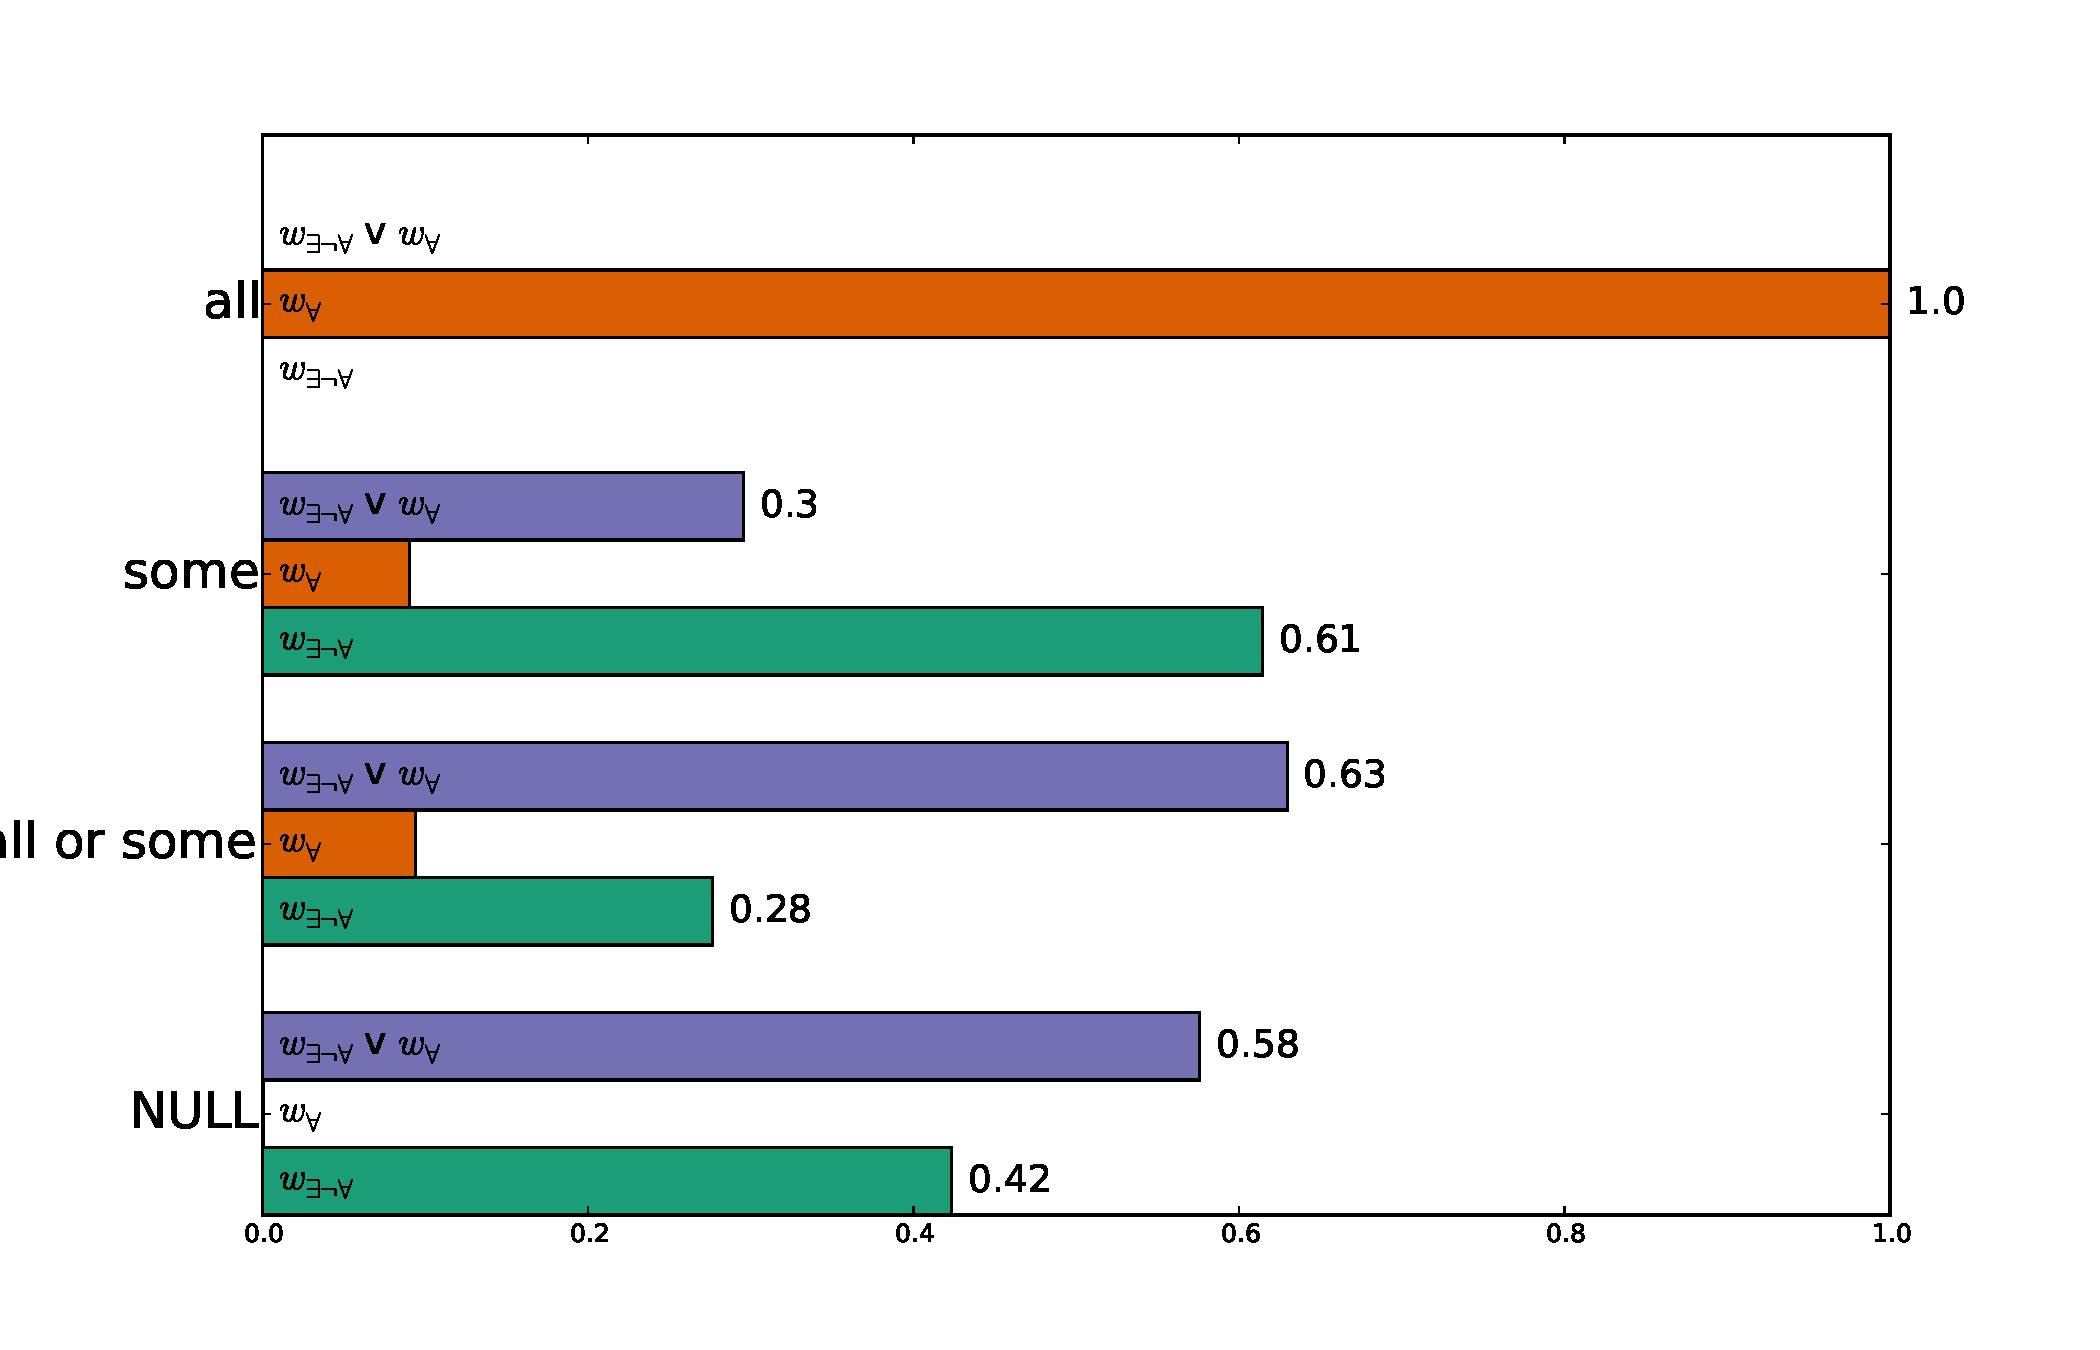
\includegraphics[width=0.5\textwidth]{fig/scalar-expertise-listener-marginalized}

\item $\SpeakerK[3]$

  $\mspace{-60mu}$
  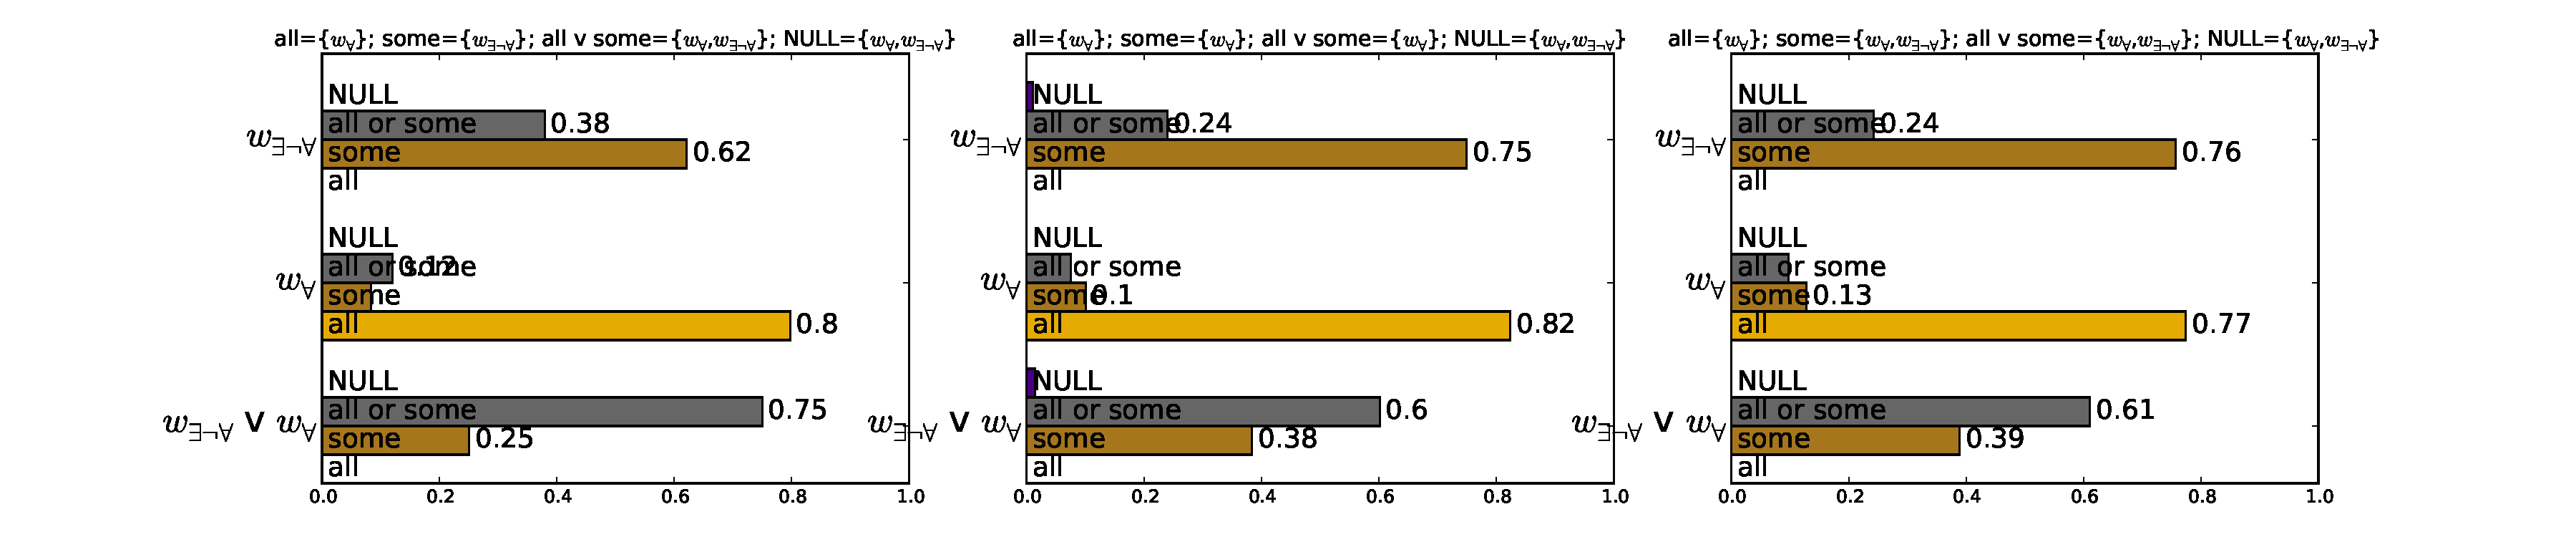
\includegraphics[width=1.2\textwidth]{fig/scalar-expertise-speaker}

\item $\SpeakerK[3]$ summed over lexica and renormalized:

  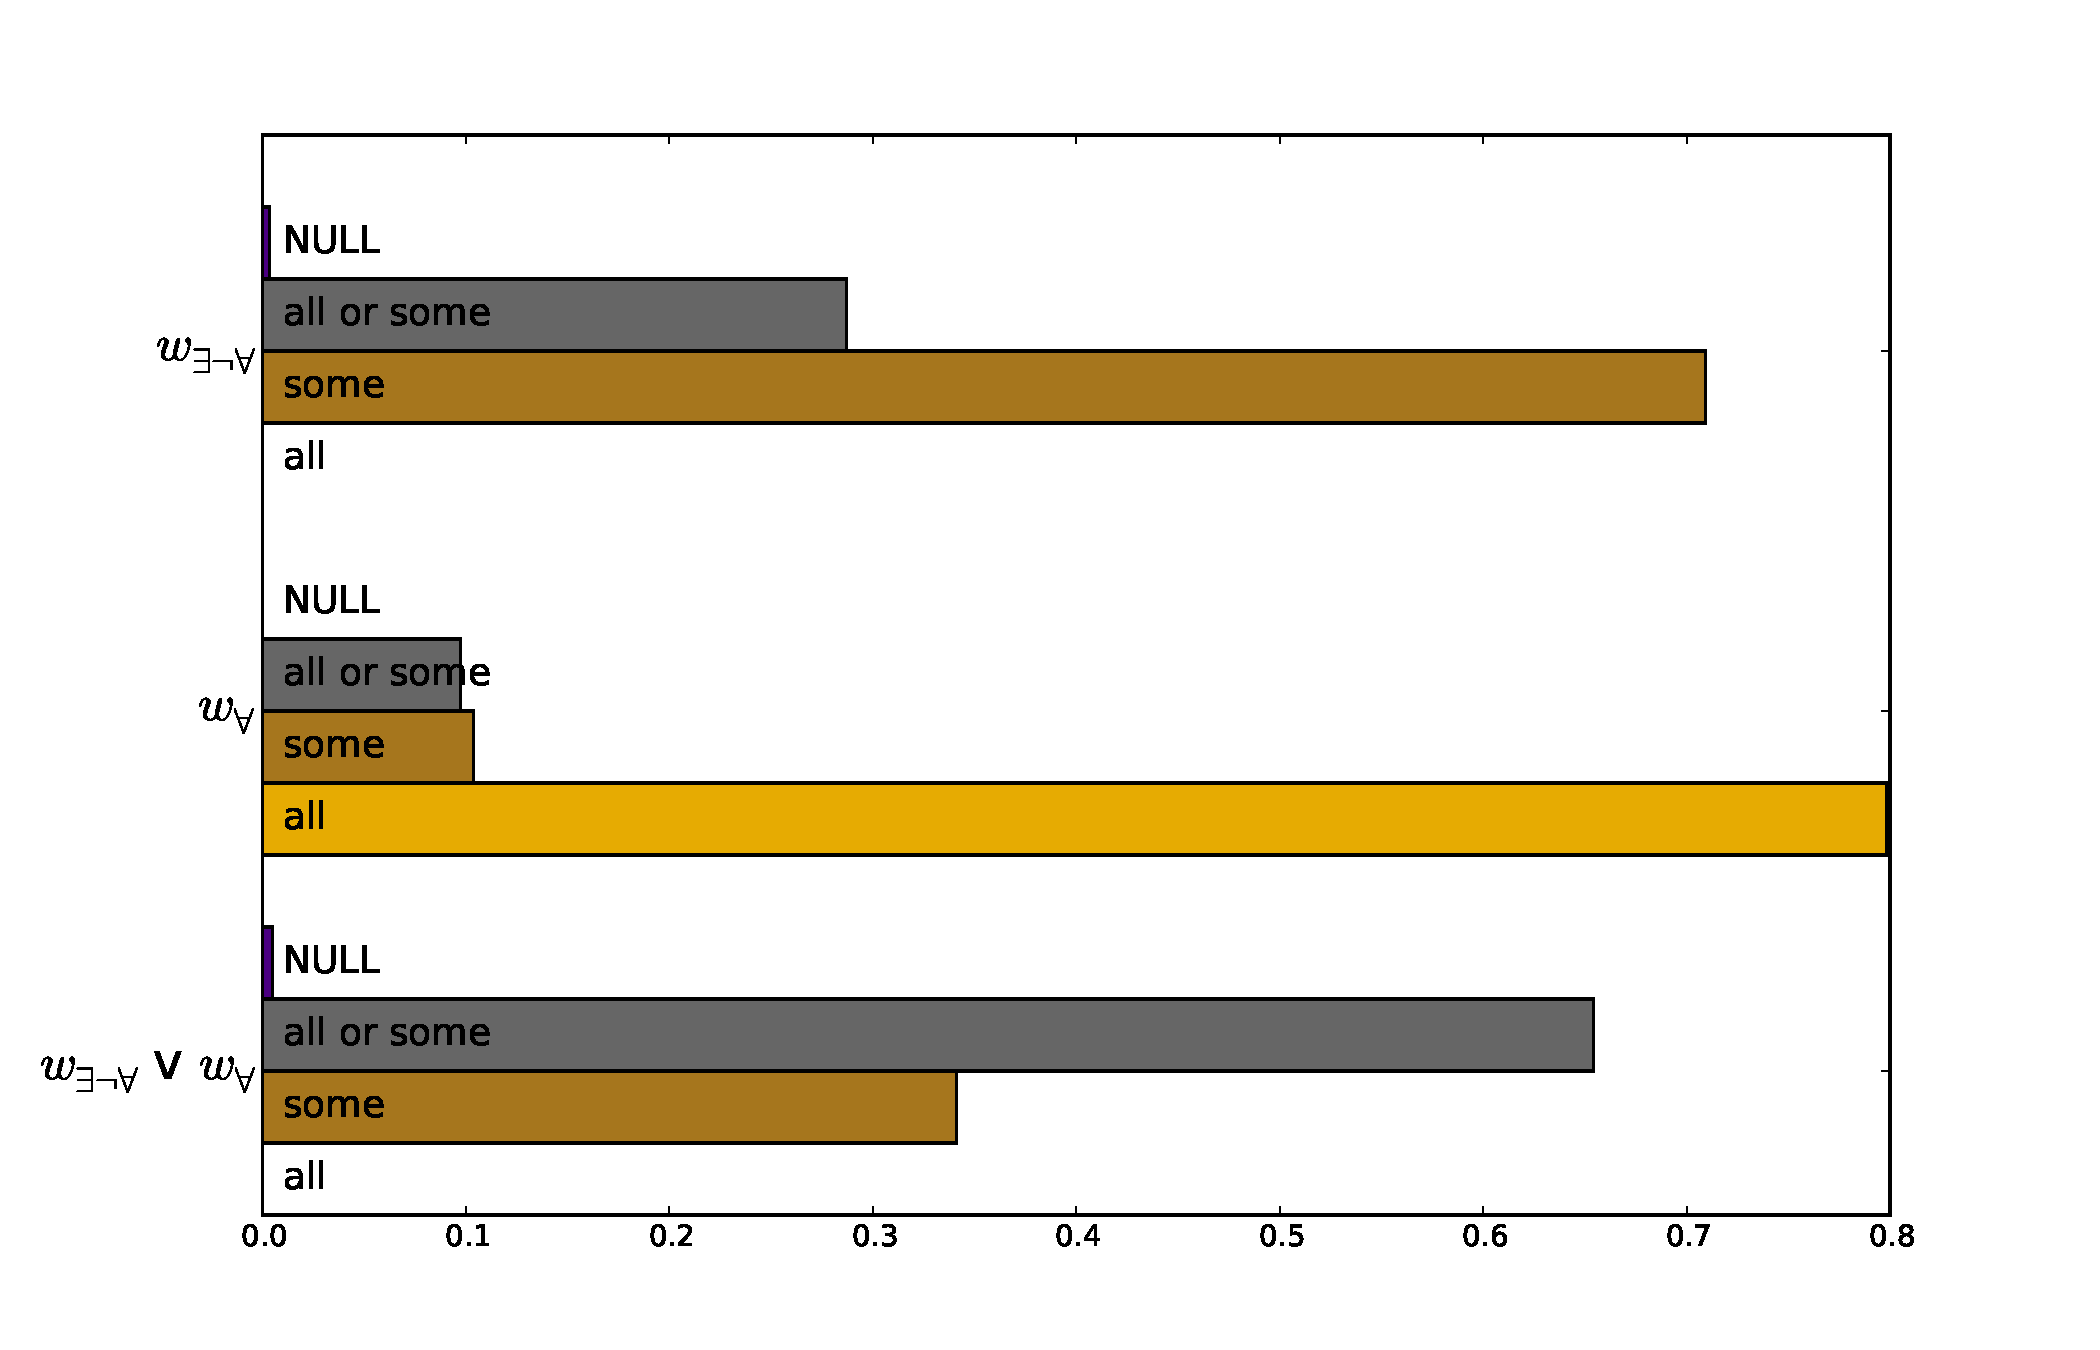
\includegraphics[width=0.5\textwidth]{fig/scalar-expertise-speaker-lexsum}
\end{examples}

\subsubsection{Markedness implicature}\label{sec:markedness}

\newcommand{\mSHORT}{\textsc{SHORT}}
\newcommand{\mLONG}{\textsc{long}}

\newcommand{\mannerstate}[1]{w_{\textsc{#1}}}
\newcommand{\wFREQ}{\mannerstate{freq}}
\newcommand{\wRARE}{\mannerstate{rare}}


\newcommand{\mannerlex}[2]{
  \left[
    \begin{array}[c]{l@{ \ \mapsto \ } l}
      \mSHORT & \set{#1} \\
      \mLONG & \set{#2}
    \end{array}
  \right]}

\begin{examples}
\item $\States = \set{\wFREQ,\wRARE}$ 
\item $\Messages = \set{\mSHORT, \mLONG}$
\item $\Lex = [\mSHORT \mapsto \set{\wFREQ,\wRARE}, \mLONG \mapsto \set{\wFREQ,\wRARE}]$
\item $\Prior = [\wFREQ \mapsto 2/3, \wRARE \mapsto 1/3]$
\item $\Costs = [\mSHORT \mapsto 1, \mLONG \mapsto 2]$
\item $\alpha = 3$; $\beta = 1$; $\gamma = 1$  
\item Lexica:
  \[
  \setlength{\arraycolsep}{2pt} 
  \begin{array}[c]{l l l}
  \mannerlex{\wFREQ,\wRARE}{\wFREQ,\wRARE}
  &
  \mannerlex{\wFREQ,\wRARE}{\wFREQ}
  &
  \mannerlex{\wFREQ,\wRARE}{\wRARE}
  \\[4ex]
  \mannerlex{\wFREQ}{\wFREQ,\wRARE}
  &
  \mannerlex{\wFREQ}{\wFREQ}
  &
  \mannerlex{\wFREQ}{\wRARE}
  \\[4ex]
  \mannerlex{\wRARE}{\wFREQ,\wRARE}
  &
  \mannerlex{\wRARE}{\wFREQ}
  &
  \mannerlex{\wRARE}{\wRARE}
  \end{array}
  \]
\end{examples}

\begin{examples}
\item $\ListenerK[3]$ after marginalization over lexica

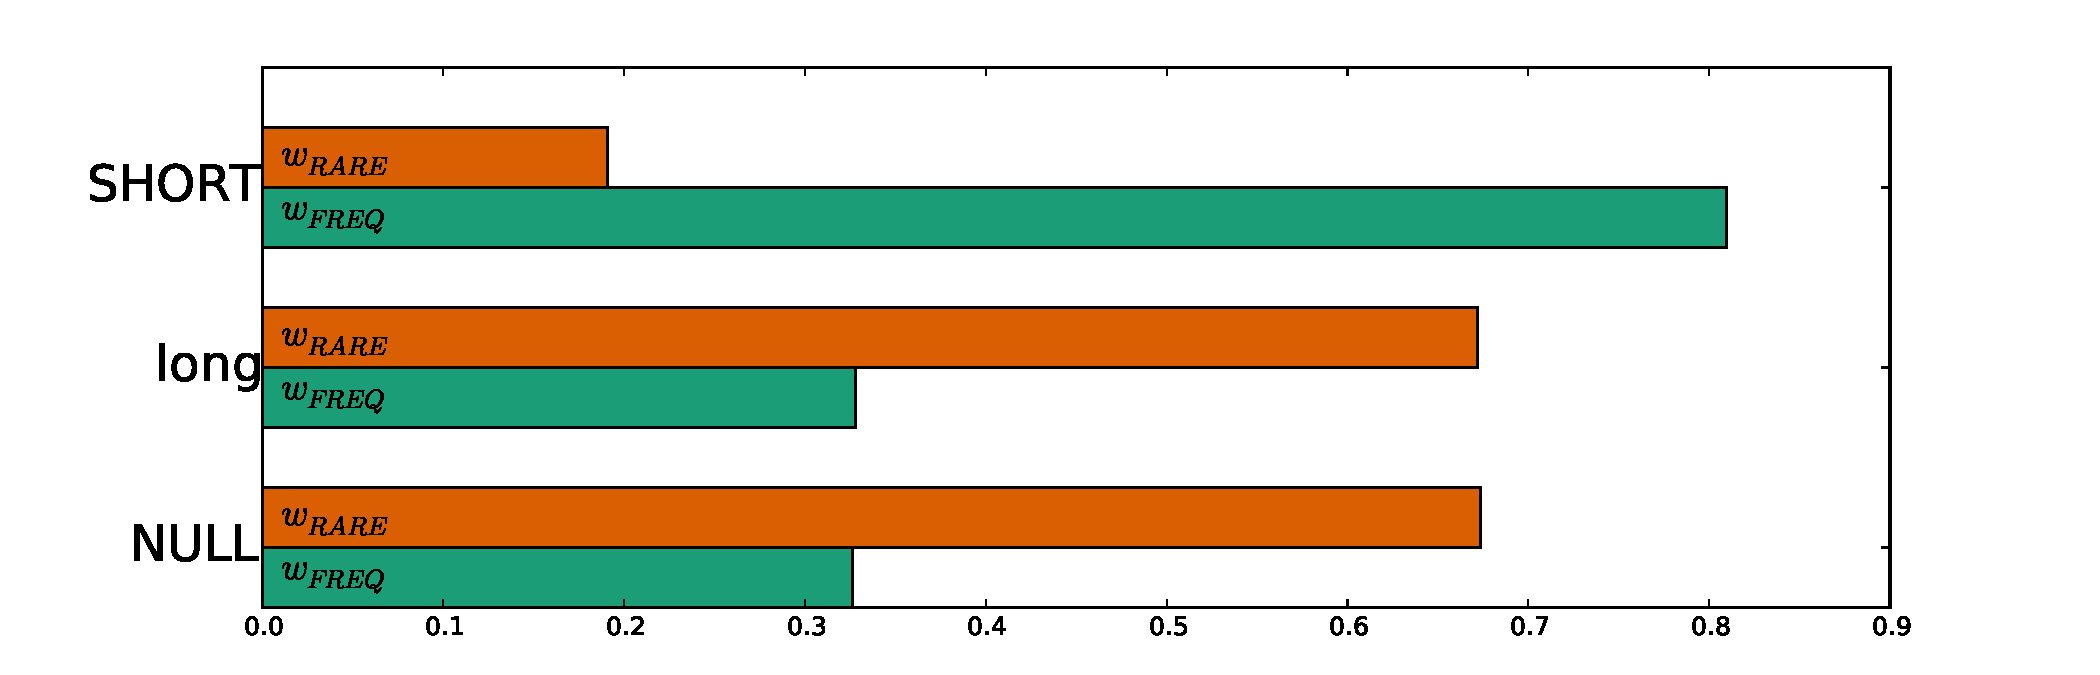
\includegraphics[width=0.5\textwidth]{fig/manner-expertise-listener-marginalized}

\item $\SpeakerK[3]$ summed over lexica and renormalized:

  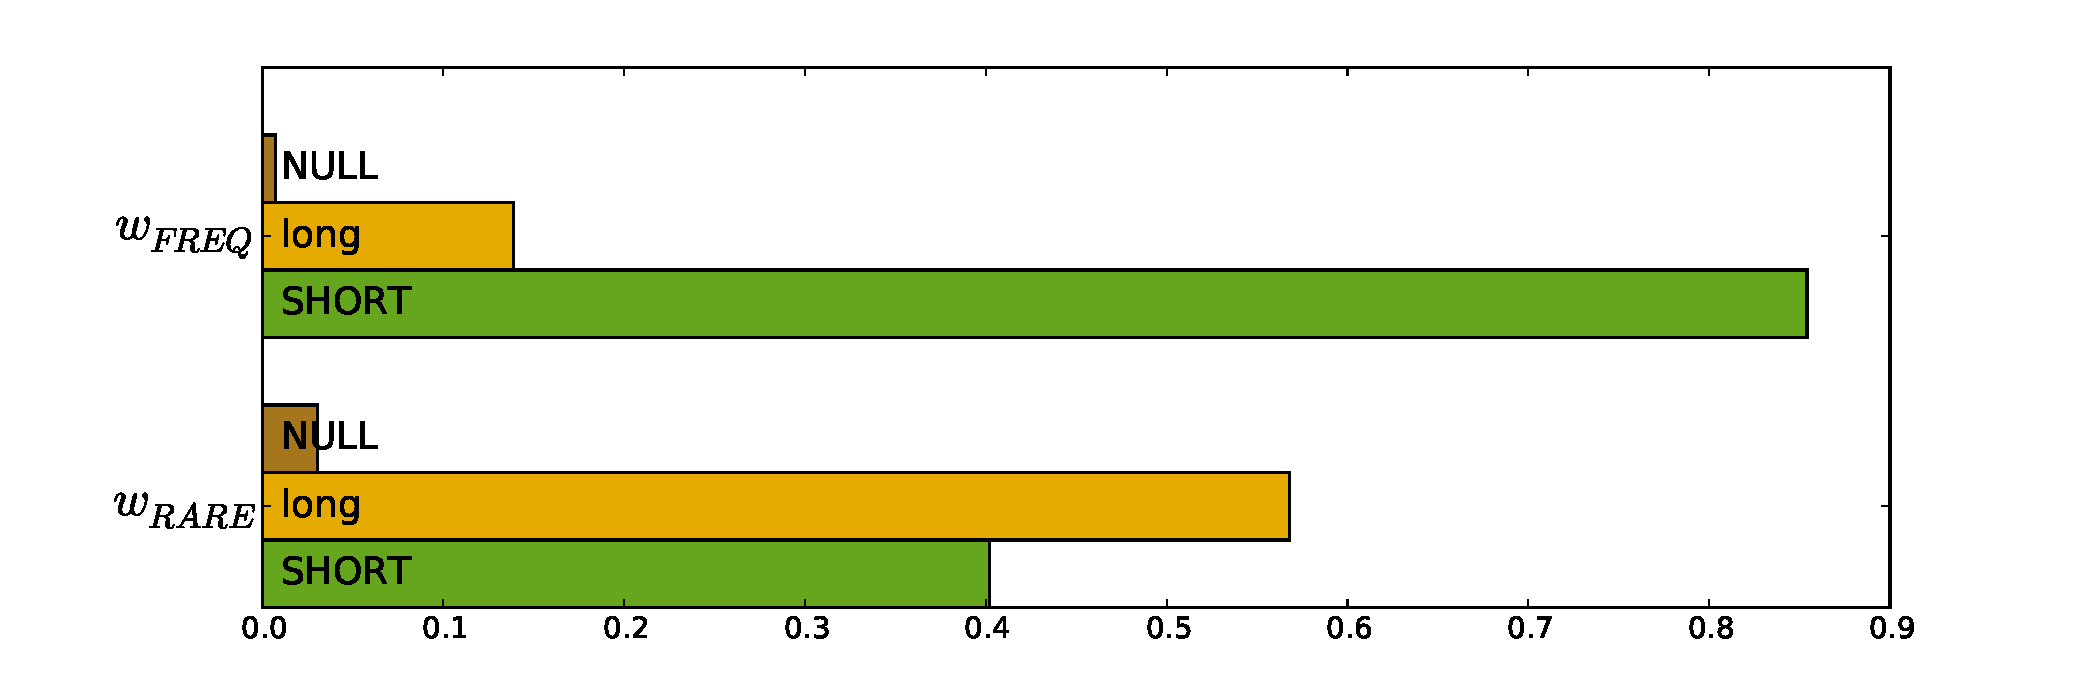
\includegraphics[width=0.5\textwidth]{fig/manner-expertise-speaker-lexsum}
\end{examples}


% The basic converational implicature (exluding \word{and}) was already
% derived by \citealt{Bergen:Goodman:Levy:2012}; our contribution is to
% extend this to the effects of HG ``violations'' and to characterizing
% where and how definitional disjunction arises.

% \citet{bergen-levy-goodman:2014} show how (i)--(ii) suffice to account
% for the Q- cases of one-way semantic inclusion described above; we
% show how they also suffice to account for the I- cases.  We show that
% adding (iii) preserves these results and permits definitional
% disjunction to arise under precisely the circumstances described
% above. On this analysis, the known disjunct serves as a \tech{focal
%   point} that the speaker and listener can coordinate on for the
% meaning of the unknown disjunct.

\subsubsection{Scalar implicture of disjunction}\label{sec:scalar-disj}

%=====================================================================

\section{Analysis}\label{sec:analysis}

\subsection{Subsumptive disjunctions}\label{sec:analysis:subsumptive}

\subsection{Definitional disjunctions}\label{sec:analysis:definitional}

\begin{examples}
\item The definitional interpretation of disjunctions such as can fall
  out of our model when the following conditions hold:
%
  \begin{itemize}
  \item it is common ground that one of the disjuncts is a
    \emph{novel} term whose meaning is known to the speaker but not to
    the listener, and that the other is known to both the speaker and
    the listener; and
  \item value is placed on the successful transmission from the
    speaker to the listener not only of the reference of the
    disjunction but also of the meaning of the novel term.
  \end{itemize}
  % 
  Under these circumstances, the meaning of the known disjunct serves
  as a \emph{focal point} that the speaker and listener can coordinate
  on for the meaning of the unknown word.
\end{examples}

%=====================================================================

\bibliographystyle{apalike}
\bibliography{levy-potts-pragdisj-bib}

\end{document}


